% Options for packages loaded elsewhere
\PassOptionsToPackage{unicode}{hyperref}
\PassOptionsToPackage{hyphens}{url}
%
\documentclass[
]{article}
\usepackage{amsmath,amssymb}
\usepackage{lmodern}
\usepackage{iftex}
\ifPDFTeX
  \usepackage[T1]{fontenc}
  \usepackage[utf8]{inputenc}
  \usepackage{textcomp} % provide euro and other symbols
\else % if luatex or xetex
  \usepackage{unicode-math}
  \defaultfontfeatures{Scale=MatchLowercase}
  \defaultfontfeatures[\rmfamily]{Ligatures=TeX,Scale=1}
\fi
% Use upquote if available, for straight quotes in verbatim environments
\IfFileExists{upquote.sty}{\usepackage{upquote}}{}
\IfFileExists{microtype.sty}{% use microtype if available
  \usepackage[]{microtype}
  \UseMicrotypeSet[protrusion]{basicmath} % disable protrusion for tt fonts
}{}
\makeatletter
\@ifundefined{KOMAClassName}{% if non-KOMA class
  \IfFileExists{parskip.sty}{%
    \usepackage{parskip}
  }{% else
    \setlength{\parindent}{0pt}
    \setlength{\parskip}{6pt plus 2pt minus 1pt}}
}{% if KOMA class
  \KOMAoptions{parskip=half}}
\makeatother
\usepackage{xcolor}
\usepackage[margin=1in]{geometry}
\usepackage{listings}
\newcommand{\passthrough}[1]{#1}
\lstset{defaultdialect=[5.3]Lua}
\lstset{defaultdialect=[x86masm]Assembler}
\usepackage{longtable,booktabs,array}
\usepackage{calc} % for calculating minipage widths
% Correct order of tables after \paragraph or \subparagraph
\usepackage{etoolbox}
\makeatletter
\patchcmd\longtable{\par}{\if@noskipsec\mbox{}\fi\par}{}{}
\makeatother
% Allow footnotes in longtable head/foot
\IfFileExists{footnotehyper.sty}{\usepackage{footnotehyper}}{\usepackage{footnote}}
\makesavenoteenv{longtable}
\usepackage{graphicx}
\makeatletter
\def\maxwidth{\ifdim\Gin@nat@width>\linewidth\linewidth\else\Gin@nat@width\fi}
\def\maxheight{\ifdim\Gin@nat@height>\textheight\textheight\else\Gin@nat@height\fi}
\makeatother
% Scale images if necessary, so that they will not overflow the page
% margins by default, and it is still possible to overwrite the defaults
% using explicit options in \includegraphics[width, height, ...]{}
\setkeys{Gin}{width=\maxwidth,height=\maxheight,keepaspectratio}
% Set default figure placement to htbp
\makeatletter
\def\fps@figure{htbp}
\makeatother
\setlength{\emergencystretch}{3em} % prevent overfull lines
\providecommand{\tightlist}{%
  \setlength{\itemsep}{0pt}\setlength{\parskip}{0pt}}
\setcounter{secnumdepth}{5}
\usepackage{booktabs}
\usepackage{setspace}
\onehalfspacing
\usepackage{xcolor}
\ifLuaTeX
  \usepackage{selnolig}  % disable illegal ligatures
\fi
\IfFileExists{bookmark.sty}{\usepackage{bookmark}}{\usepackage{hyperref}}
\IfFileExists{xurl.sty}{\usepackage{xurl}}{} % add URL line breaks if available
\urlstyle{same} % disable monospaced font for URLs
\hypersetup{
  hidelinks,
  pdfcreator={LaTeX via pandoc}}

\author{}
\date{\vspace{-2.5em}}

\begin{document}

{
\setcounter{tocdepth}{2}
\tableofcontents
}
\hypertarget{MIKK-F2-chap}{%
\section{Genetic linkage study of bold/shy behaviours in the MIKK panel}\label{MIKK-F2-chap}}

The purpose of the study described in this chapter was to run the behavioural analysis described in Chapter \ref{Pilot-chap} over the MIKK panel described in Chapter \ref{MIKK-genomes-chap}, identify the lines that diverged in both their behaviour, and the level of transmission of their behaviour onto their \emph{\definecolor{iCab_424B4D}{HTML}{424B4D}\textcolor{iCab_424B4D}{iCab}} reference tank partner, and then use them as the parental strains in an F2 cross to attempt to identify the genetic variants associated with those differences. \definecolor{18-2_FF66A6}{HTML}{FF66A6}\textcolor{18-2_FF66A6}{18-2}

\hypertarget{MIKK-F2-cross}{%
\subsection{The F2 cross experimental setup}\label{MIKK-F2-cross}}

The F2 cross is a traditional method for mapping genetic variants associated with traits of interest. A schema for the method is presented in \textbf{Figure \ref{fig:F2-cross-schema}}. In essence, it involves starting with two inbred strains that diverge for the trait of interest (the `parental strains', or F0 generation F0). One then crosses the parental strains to create a generation of F1 hybrid individuals who each possess, for every pair of their chromosomes, one chromosome from each of their parents. The individuals in this F1 generation are genetically identical to their parents with respect to their germ line. Finally, one inter-crosses the F1 generation to create a set of F2 individuals that share unique combinations of the original F0 strains' genotypes, and tend to display values for the trait of interest that span across the spectrum between the extreme values of their parents.



\begin{figure}
\includegraphics[width=1\linewidth]{figs/mikk_behaviour/F2-cross-schema} \caption{Schema of the F2-cross experimental setup. The F0 generation comprises two medaka strains that have extreme, opposing values for a trait of interest, represented by the colours red and blue. Below them is an illustrative single pair of chromosomes. The chromosomes within each pair are depicted as the same colour, as the strains are homozygous through successive generations of inbreeding. Their F1 offspring is heterozygous for each pair of their 24 chromosomes, and all F1 individuals are therefore almost genetically identical to one another (with the exception of somatic mutations and the regions of the genome that were not homozygous in the parental generations). The F1 individuals are then inter-crossed with one another to produce the F2 generation, which, due to recombination events during gamete formation, have unique combinations of the parental strains' genotypes, and tend to span the phenotypic spectrum between the extremes of their F0 parental strains, represented by their colours.}\label{fig:F2-cross-schema}
\end{figure}

\hypertarget{data-collection---f0-generation}{%
\subsection{Data collection - F0 generation}\label{data-collection---f0-generation}}

In November 2019 I traveled to the fish facility managed by our collaborator, Felix Loosli at KIT in Karlsruhe, and over the course of 11 days from 11 to 21 November 2019, I ran the behavioural assay described in Chapter \ref{pilot-data-collection} another 206 times. I again used the \emph{\definecolor{iCab_424B4D}{HTML}{424B4D}\textcolor{iCab_424B4D}{iCab}} strain as the reference fish, and for the test fish I used either an individual from one of the MIKK panel lines, individuals captured from the same Kiyosu population as the MIKK panel but permitted to breed freely within a separate tank in the facility (`Kiyosu closed-capture', or `Kiyosu CC'), or individuals from a related but different species of medaka from the Philippines, \emph{Oryzias luzonensis}. I ensured that I performed at least 2 assay runs for each MIKK panel line that was available, generating a minimum of 8 test fish replicates per line. As there were four pairs of fish in the test tank during each run, the complete dataset comprises 824 videos of pairs of fish, which I further divided by assay component (open field and novel object) to create 1648 videos.

I again used the software \emph{idtrackerai} {[}@romero-ferreroIdtrackerAiTracking2019{]} to track the movement of the fishes across frames of each video. After adjusting the software parameters for each video to maximise the number of frames that were successfully tracked, I was left with 1610 out of the 1648 videos (\textasciitilde97.7\%) where both fishes were tracked over at least 85\% of frames, and I only included these 1610 videos in the downstream analysis. The first question to address was whether the MIKK panel lines differed in their behaviours. I therefore computed each individual fish's mean speed (measured as the distance traveled in pixels per 0.08 seconds) over the course of the full 20-minute video, grouped them by line, and plotted the results presented in \textbf{Figure \ref{fig:mikk-mean-speed}}. I continue to use the same order and colour palette for the MIKK panel lines as in this Figure throughout the rest of this Chapter.



\begin{figure}
\includegraphics[width=1\linewidth]{figs/mikk_behaviour/F0_line_mean_speed_0.08} \caption{Mean speed of the MIKK panel and other strains over the course of the entire 20-minute video (measured as the distance traveled in pixels per 0.05 seconds). \emph{\definecolor{iCab_424B4D}{HTML}{424B4D}\textcolor{iCab_424B4D}{iCab}} fishes in the \emph{\definecolor{iCab_424B4D}{HTML}{424B4D}\textcolor{iCab_424B4D}{iCab}}-\emph{\definecolor{iCab_424B4D}{HTML}{424B4D}\textcolor{iCab_424B4D}{iCab}} control condition are at the top, the MIKK panel lines are sorted by their group median, and the Kiyosu closed capture and \emph{O. luzonensis} fishes are at the bottom.}\label{fig:mikk-mean-speed}
\end{figure}

This figure shows that there are clear differences between some MIKK panel lines at the extremes, and that the lines differ in the amount of within-line variance observed. This figure acted as a guide to determine which lines to select as the parental strains in the F2 cross. To identify genetic variants directly associated with bold-shy behaviours, I sought to select lines that showed either high or low levels of movement, and preferably low within-line variance.



\begin{figure}
\includegraphics[width=1\linewidth]{figs/mikk_behaviour/line_mean_speed_variance_0.05_all} \caption{Line median (vertical axis) and line variance (horizontal axis) for individual mean speed across the full 20-minute video (i.e.~both the open field and novel object assay components).}\label{fig:mikk-mean-speed-variance}
\end{figure}

\hypertarget{hmm-states}{%
\subsection{HMM states}\label{hmm-states}}

To examine these behaviours at a finer resolution, as for the pilot study described in \ref{Pilot-chap}, I again applied a hidden markov model (\textbf{HMM}) to classify the fishes' movements based on their distance and angle of travel between time intervals. I used the same method to select the best choice of time interval and number of states (\textbf{Figure \ref{mikk-param-comp}}). Here I observed the same phenomenon where the parameter combinations that performed the best showed an asymmetry between some states that would make interpretation difficult. For example, a time interval of 0.08 seconds combined with a state space of 17 caused state 4 to appear to get carved out of state 3 (\textbf{Figure \ref{fig:mikk-hmm-asym}}).



\begin{figure}
\includegraphics[width=1\linewidth]{figs/mikk_behaviour/compare_params} \caption{Comparison between HMM parameters. Horizontal axis: Mean concordance between states assigned by HMMs through a 2-fold cross-validation process. Vertical axis: Kruskal-Wallis statistic comparing strains based on the proportion of time spent in each HMM state, summed across all states. Size of points correspond to the interval, in seconds, between which the distance and angle of travel was calculated (Methods).}\label{fig:mikk-param-comp}
\end{figure}



\begin{figure}
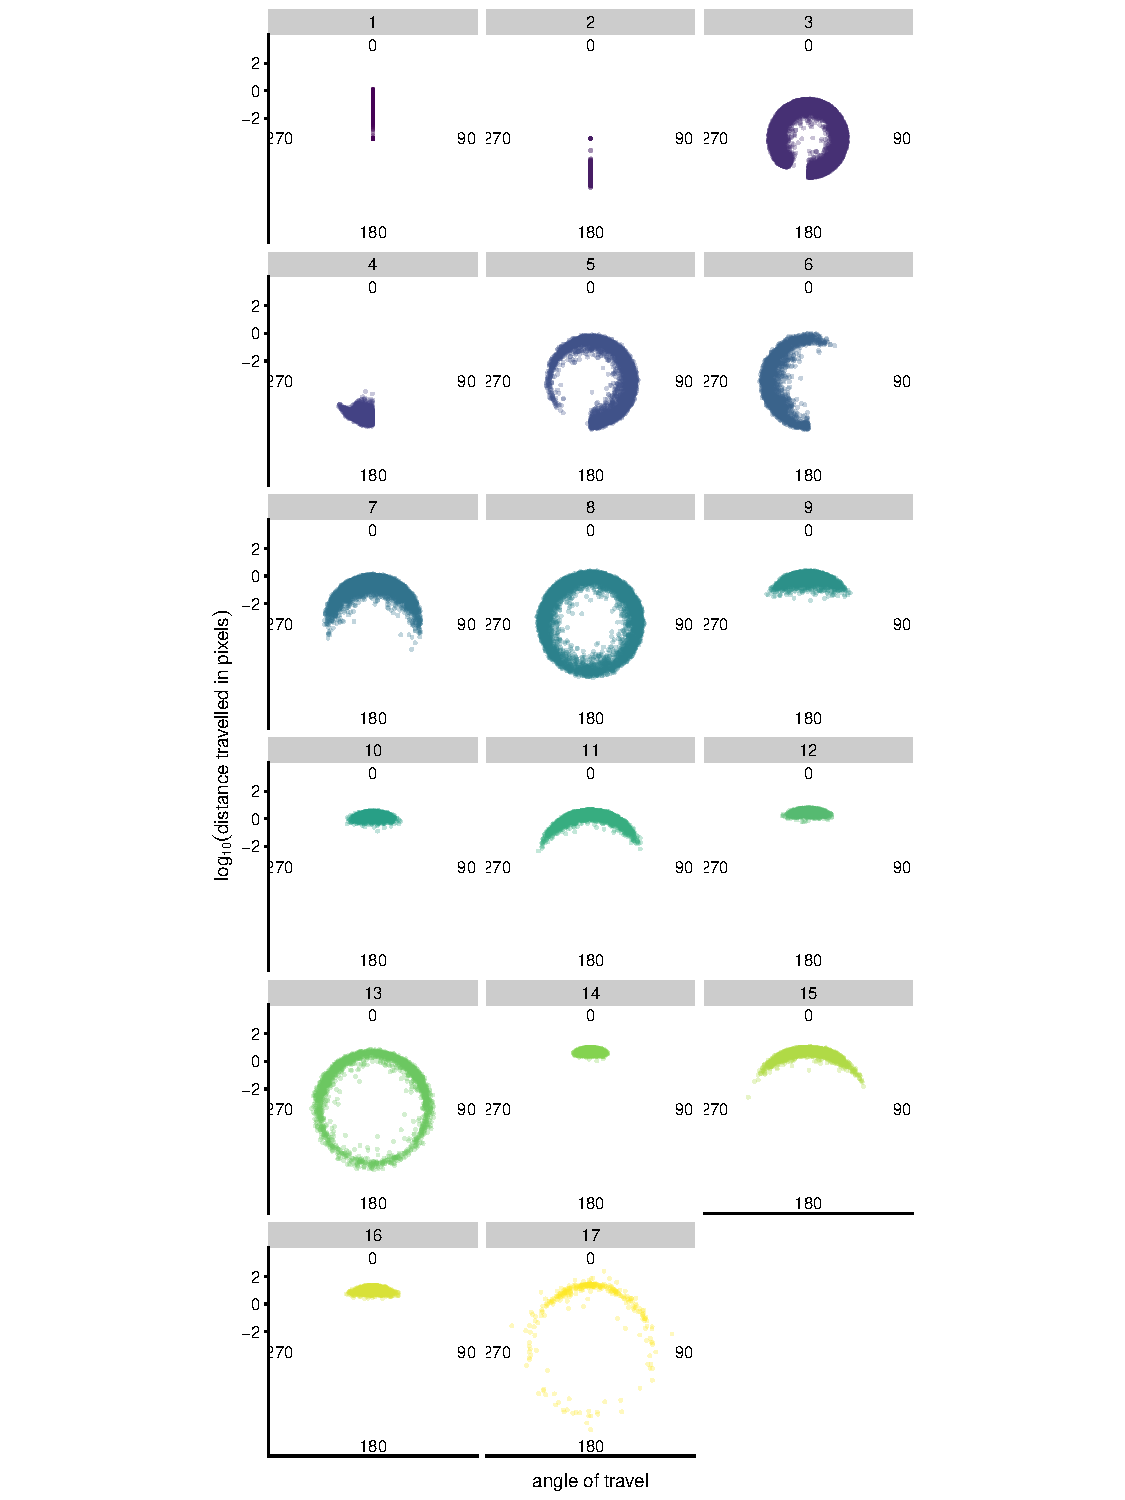
\includegraphics[width=1\linewidth]{figs/mikk_behaviour/0.08_17_polar_all_dge} \caption{The best apparent combination of parameters (0.08 time interval with a 17-state space) created an asymmetry between states 3 and 4, which would causes difficulties in interpreting their biological relevance.}\label{fig:mikk-hmm-asym}
\end{figure}

The best combination of parameters without this asymmetry was a time interval of 0.05 seconds with a state space of 15 (see the polar plots for the states in \textbf{Appendix @ref(fig:hmm-states-0.05)}). However, due to a glitch in the video recording software, several videos recorded on 13 November 2019 were incorrectly recorded with a frame rate of 14 instead of the desired 30. The insufficient number of frames for those videos meant that it was impossible to measure the distance and angle of travel between a time interval as low as 0.05 seconds. So that these videos could be included in the dataset, I accordingly selected the combination of 15 states and a 0.08-second interval for all downstream analyses.



\begin{figure}
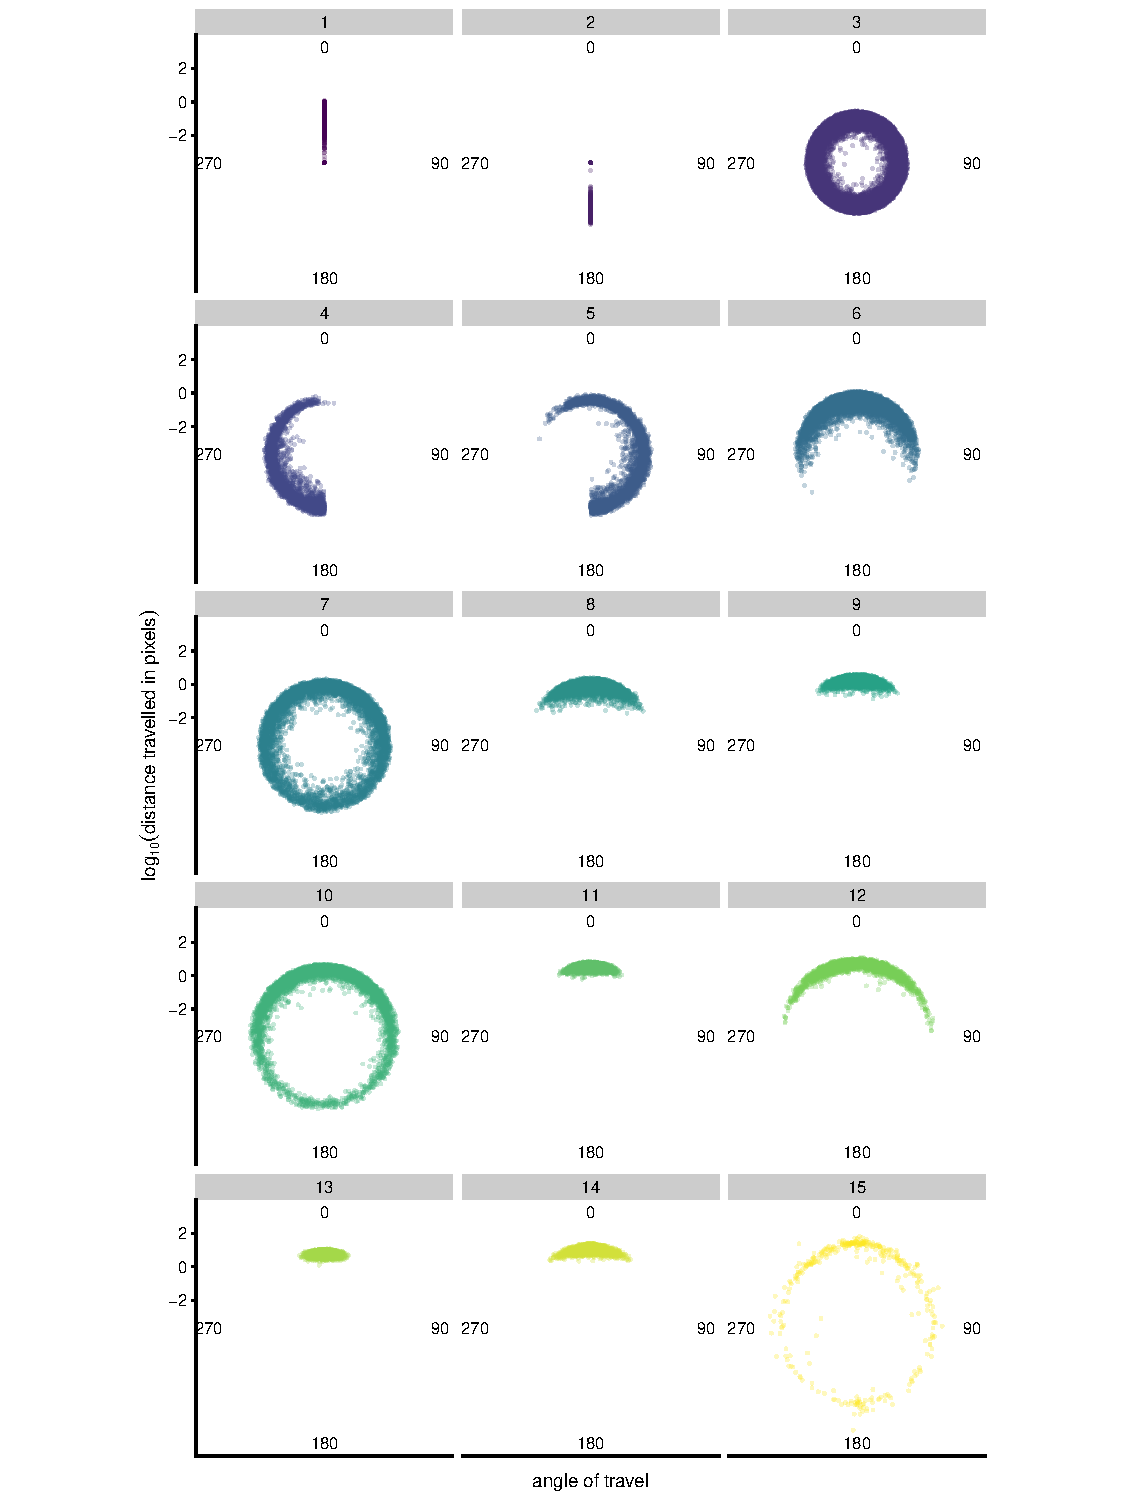
\includegraphics[width=1\linewidth]{figs/mikk_behaviour/0.08_15_polar_all_dge} \caption{The HMM states used for the downstream analysis, with the model classified based on the distance of travel (log\textsubscript{10} pixels, radial axis) and angle of travel (angle). A straight forward movement would sit around 0°, a left movement around 270°, and a right movement around 90°.}\label{fig:mikk-hmm-sym}
\end{figure}

\hypertarget{social-genetic-effects}{%
\subsection{Social genetic effects}\label{social-genetic-effects}}

As discussed above, in this project our traits of interest include not only direct genetic behaviours, but also social genetic behaviours. We therefore sought to identify the MIKK panel lines that transmitted their behaviour onto the reference \emph{\definecolor{iCab_424B4D}{HTML}{424B4D}\textcolor{iCab_424B4D}{iCab}} tank partners either to the largest or smallest degrees. I formulated two methods to measure this, referred to as a) HMM state co-occupancy; and b) reference deviation. The first, HMM state co-occupancy, measured the proportions of time that the \emph{\definecolor{iCab_424B4D}{HTML}{424B4D}\textcolor{iCab_424B4D}{iCab}} reference fish spent in the same HMM state as its tank partner. The second, deviation of the reference fishes' deviation from the behaviour exhibited in the control condition, seeks to quantify the extent to which the \emph{\definecolor{iCab_424B4D}{HTML}{424B4D}\textcolor{iCab_424B4D}{iCab}}'s behaviour changes when partnered with

\hypertarget{state-co-occupancy}{%
\subsubsection{State co-occupancy}\label{state-co-occupancy}}

\textbf{Figure \ref{fig:F0-sge-cooc-box}} sets out the proportions of total time for each assay sub-component that each pair of individual fish spent in the same HMM state, grouped by line and ranked in the same order as their group median for individual mean speed as shown above in \textbf{Figure \ref{fig:mikk-mean-speed}}. \textbf{\ref{fig:F0-sge-cooc-box}A} shows the data as boxplots, with \(p\)-values from the Kruskal-Wallis test comparing all groups. \textbf{Figure \ref{fig:F0-sge-cooc-box}B} shows the same data but with each group's median represented by columns to make it easier to compare group medians. Of the slower-moving lines, \definecolor{8-2_FF699C}{HTML}{FF699C}\textcolor{8-2_FF699C}{8-2} and \definecolor{18-2_FF66A6}{HTML}{FF66A6}\textcolor{18-2_FF66A6}{18-2} tend to show relatively higher state co-occupancy in the open field component, but during the novel object component, the slow-moving line \definecolor{139-4_FF61CC}{HTML}{FF61CC}\textcolor{139-4_FF61CC}{139-4} has the highest median co-occupancy of all lines. Of the faster-moving lines, \definecolor{43-2_F17D50}{HTML}{F17D50}\textcolor{43-2_F17D50}{43-2} and \definecolor{13-2_F57A5F}{HTML}{F57A5F}\textcolor{13-2_F57A5F}{13-2} showed the highest state co-occupancy during the open field assay component. However, the moderate-to-fast line \definecolor{21-2_49B500}{HTML}{49B500}\textcolor{21-2_49B500}{21-2} had relatively high state co-occupancy during both assay components.



\begin{figure}
\includegraphics[width=1\linewidth]{figs/mikk_behaviour/0.08_15_cooc_box_all} \caption{Frequency of HMM state co-occupancy}\label{fig:F0-sge-cooc-box}
\end{figure}

To visualise which states are driving the higher co-occupancy measures, for a selection of lines I generated a heatmap of the states occupied simultaneously by the \emph{\definecolor{iCab_424B4D}{HTML}{424B4D}\textcolor{iCab_424B4D}{iCab}} reference and MIKK test fishes, combining the observations for all individuals within each test fish group (\textbf{Figure \ref{fig:F0-sge-cooc-heat}}). When \emph{\definecolor{iCab_424B4D}{HTML}{424B4D}\textcolor{iCab_424B4D}{iCab}} is paired with \definecolor{18-2_FF66A6}{HTML}{FF66A6}\textcolor{18-2_FF66A6}{18-2} or \definecolor{8-2_FF699C}{HTML}{FF699C}\textcolor{8-2_FF699C}{8-2}, the fishes most frequently occupy states 3 or 1 in both open field and novel object components. In pairings with line \definecolor{139-4_FF61CC}{HTML}{FF61CC}\textcolor{139-4_FF61CC}{139-4}, while the test fishes remain in the still states 1 or 3 during the open field assay, \emph{\definecolor{iCab_424B4D}{HTML}{424B4D}\textcolor{iCab_424B4D}{iCab}} tends to be moving much faster in states 11 and 13. However, during the novel object component, they co-occupy state 3 more than in any other combination. This general pattern is observed with line \definecolor{14-2_F066EA}{HTML}{F066EA}\textcolor{14-2_F066EA}{14-2} as well, albeit to a lesser extent. For \definecolor{38-2_00C08B}{HTML}{00C08B}\textcolor{38-2_00C08B}{38-2}, the fishes tend not to show a strong preference for co-occupying a particular state for either assay component, but the diagonal spread indicates that they tend to move at similar speeds. When paired with the faster moving \definecolor{21-2_49B500}{HTML}{49B500}\textcolor{21-2_49B500}{21-2}, the novel object component appears to accentuate the co-occupancy of state 3 that is also observed in the open field component. Finally, when paired with line \definecolor{40-1_93AA00}{HTML}{93AA00}\textcolor{40-1_93AA00}{40-1}, in both assay components, both fishes show a strong preference for the faster-moving states.



\begin{figure}
\includegraphics[width=1\linewidth]{figs/mikk_behaviour/0.08_15_cooc_heatmap} \caption{Heatmaps for a selection of MIKK panel lines (including those ultimately selected as the parental strains in the F2 cross) showing the frequency of HMM states simultaneously occupied by the reference (x-axis) and test (y-axis) fishes, aggregated over all replicates in each line.}\label{fig:F0-sge-cooc-heat}
\end{figure}

\hypertarget{deviation-of-from-its-control-condition}{%
\subsubsection{\texorpdfstring{Deviation of \emph{\definecolor{iCab_424B4D}{HTML}{424B4D}\textcolor{iCab_424B4D}{iCab}} from its control condition}{Deviation of  from its control condition}}\label{deviation-of-from-its-control-condition}}

The second method for quantifying the level of behavioural transmission from test fish to \emph{\definecolor{iCab_424B4D}{HTML}{424B4D}\textcolor{iCab_424B4D}{iCab}} reference fish was to determine the proportion of time that the \emph{\definecolor{iCab_424B4D}{HTML}{424B4D}\textcolor{iCab_424B4D}{iCab}} spent in a particular state when paired with another \emph{\definecolor{iCab_424B4D}{HTML}{424B4D}\textcolor{iCab_424B4D}{iCab}}, and then quantify the degree to which those proportions change when in the presence of a fish from another line (\textbf{Figure \ref{fig:F0-sge-deviation}}). \textbf{Figure \ref{fig:F0-sge-deviation}A} presents boxplots for state frequencies for all \emph{\definecolor{iCab_424B4D}{HTML}{424B4D}\textcolor{iCab_424B4D}{iCab}} individuals in \emph{\definecolor{iCab_424B4D}{HTML}{424B4D}\textcolor{iCab_424B4D}{iCab}}-\emph{\definecolor{iCab_424B4D}{HTML}{424B4D}\textcolor{iCab_424B4D}{iCab}} pairings. I further calculated the state frequencies for all \emph{\definecolor{iCab_424B4D}{HTML}{424B4D}\textcolor{iCab_424B4D}{iCab}} reference fishes for all other MIKK line pairings. For each combination of assay component, line-pairing, and HMM state, I then ran Welch's t-test {[}@ruxtonUnequalVarianceTtest2006{]} comparing the proportions of time the \emph{\definecolor{iCab_424B4D}{HTML}{424B4D}\textcolor{iCab_424B4D}{iCab}} individuals spent in that state when paired with another \emph{\definecolor{iCab_424B4D}{HTML}{424B4D}\textcolor{iCab_424B4D}{iCab}}, against the proportions of time the \emph{\definecolor{iCab_424B4D}{HTML}{424B4D}\textcolor{iCab_424B4D}{iCab}} reference individuals spent in that state when paired with a different MIKK line. I then summed the t-statistics across states to generate a single metric for each combination of line and assay component, and plotted the results in \textbf{Figure \ref{fig:F0-sge-deviation}B}.



\begin{figure}
\includegraphics[width=1\linewidth]{figs/mikk_behaviour/0.08_15_deviation} \caption{Deviation of state frequency for \emph{\definecolor{iCab_424B4D}{HTML}{424B4D}\textcolor{iCab_424B4D}{iCab}} reference fishes when paired with MIKK panel lines relative to when paired with another \emph{\definecolor{iCab_424B4D}{HTML}{424B4D}\textcolor{iCab_424B4D}{iCab}}. \textbf{A}: Boxplots of HMM state frequency for \emph{\definecolor{iCab_424B4D}{HTML}{424B4D}\textcolor{iCab_424B4D}{iCab}} individuals when paired with another \emph{\definecolor{iCab_424B4D}{HTML}{424B4D}\textcolor{iCab_424B4D}{iCab}}. \textbf{B}:}\label{fig:F0-sge-deviation}
\end{figure}

The first thing to note in this Figure is that \emph{\definecolor{iCab_424B4D}{HTML}{424B4D}\textcolor{iCab_424B4D}{iCab}}'s deviations from its behaviour exhibited in the control condition tend to be smaller when paired with faster-moving fishes. This was expected given \emph{\definecolor{iCab_424B4D}{HTML}{424B4D}\textcolor{iCab_424B4D}{iCab}} is also a faster-moving fish, but it strengthens the observation that when paired with slower-moving fishes, those tank partners are causing the \emph{\definecolor{iCab_424B4D}{HTML}{424B4D}\textcolor{iCab_424B4D}{iCab}} reference fish to move slower than they would otherwise. Of the slower-moving MIKK lines, \definecolor{4-2_FC61D4}{HTML}{FC61D4}\textcolor{4-2_FC61D4}{4-2} and \definecolor{14-2_F066EA}{HTML}{F066EA}\textcolor{14-2_F066EA}{14-2} causing the largest deviations of the \emph{\definecolor{iCab_424B4D}{HTML}{424B4D}\textcolor{iCab_424B4D}{iCab}} reference fishes' behaviours from their control condition behaviour in the open field and novel object components respectively. I also observe large deviations for the moderately-moving \definecolor{106-2_00B9E3}{HTML}{00B9E3}\textcolor{106-2_00B9E3}{106-2} and \definecolor{71-1_00BECD}{HTML}{00BECD}\textcolor{71-1_00BECD}{71-1} during the novel object components. There are no clear outliers for either assay component for any of the faster moving lines.

\hypertarget{selection-of-lines-for-the-f2-cross}{%
\subsection{Selection of lines for the F2 cross}\label{selection-of-lines-for-the-f2-cross}}

On the basis of the above findings, I selected 6 MIKK panel lines as the parental lines for the F2 cross (\textbf{Figure @ref(F0-line-mean-speed-select}). Conceptually, I sought to select lines that diverged on two measures: a) bold-shy behaviours; and b) the extent to which the lines transmitted their behaviours onto their tank partners. As \emph{\definecolor{iCab_424B4D}{HTML}{424B4D}\textcolor{iCab_424B4D}{iCab}} is a fast-moving line, it was more difficult to detect instances where fast-moving MIKK panel lines were influencing its behaviour. I was therefore more confident of identifying slow-movement/high-charisma lines, and so to increase the likelihood of identifying genetic variants that are responsible for a stronger transmission of slow-moving behaviours, I chose two slow-movement/high-charisma lines for the F2 cross: \definecolor{18-2_FF66A6}{HTML}{FF66A6}\textcolor{18-2_FF66A6}{18-2} and \definecolor{8-2_FF699C}{HTML}{FF699C}\textcolor{8-2_FF699C}{8-2}. In the event that both lines possessed the same genetic variants that influence this behavioural transmission trait, it would vastly increase the power of detecting it during the genetic linkage analysis. Both these lines were one of the most slow-moving lines, had high levels of state co-occupancy during both assay components, and \definecolor{18-2_FF66A6}{HTML}{FF66A6}\textcolor{18-2_FF66A6}{18-2} caused a high level of deviation from the \emph{\definecolor{iCab_424B4D}{HTML}{424B4D}\textcolor{iCab_424B4D}{iCab}} control condition.

\begin{figure}
\includegraphics[width=1\linewidth]{figs/mikk_behaviour/line_mean_speed_0.05_selected} \caption{(ref:F0-line-mean-speed-select)}\label{fig:F0-line-mean-speed-select}
\end{figure}

For the slow-movement/low-charisma line, I selected \definecolor{50-2_BB81FF}{HTML}{BB81FF}\textcolor{50-2_BB81FF}{50-2} which exhibited a moderately slow level of movement, low within-line variance for mean speed, and low measures for both state co-occupancy and \emph{\definecolor{iCab_424B4D}{HTML}{424B4D}\textcolor{iCab_424B4D}{iCab}} deviation. For the high-movement/high-charisma line, I selected \definecolor{21-2_49B500}{HTML}{49B500}\textcolor{21-2_49B500}{21-2}. Despite its high within line variance (\textbf{Figure \ref{fig:F2-time-dge-of}}), this potentially made it easier to detect its social genetic effects, as the slower-moving individuals appeared to transmit those behaviours strongly to their \emph{\definecolor{iCab_424B4D}{HTML}{424B4D}\textcolor{iCab_424B4D}{iCab}} tank partners, giving it a high score among fast-moving lines for state co-occupancy across both assay components. For the high-movement/low-charisma line I selected \definecolor{40-1_93AA00}{HTML}{93AA00}\textcolor{40-1_93AA00}{40-1}, as it has low within-line variance, and low-to-moderate metrics for state co-occupancy and \emph{\definecolor{iCab_424B4D}{HTML}{424B4D}\textcolor{iCab_424B4D}{iCab}} deviation. However, I note that these measures may be confounded by the possibility that \definecolor{40-1_93AA00}{HTML}{93AA00}\textcolor{40-1_93AA00}{40-1} behaves in a similar way to \emph{\definecolor{iCab_424B4D}{HTML}{424B4D}\textcolor{iCab_424B4D}{iCab}}, which would be difficult to determine whether it was behaving differently.

In addition to these extreme lines, I also selected a line that was intermediate for both traits in an attempt to avoid breeding incompatibilities that might arise from attempting to cross lines with such divergent behavioural traits. For this purpose I selected line \definecolor{38-2_00C08B}{HTML}{00C08B}\textcolor{38-2_00C08B}{38-2} for its intermediate speed, low within-line variance for mean speed, and intermediate measures for HMM state co-occupancy and \emph{\definecolor{iCab_424B4D}{HTML}{424B4D}\textcolor{iCab_424B4D}{iCab}} deviation.



\begin{figure}
\includegraphics[width=1\linewidth]{figs/mikk_behaviour/line_mean_speed_variance_selected} \caption{Line median (vertical axis) and line variance (horizontal axis) for individual mean speed across the full 20-minute video (i.e.~both the open field and novel object assay components), coloured for the lines selected as the parental strains for the F2 cross.}\label{fig:F0-line-mean-speed-var-select}
\end{figure}

\hypertarget{direct-genetic-effects}{%
\subsection{Direct genetic effects}\label{direct-genetic-effects}}

With these lines selected, I ran a similar analysis to what I described in \ref{Pilot-chap}, where I ran multi-way ANOVAs to determine whether certain lines differed in the proportions of time they spent in these HMM states, while including the date of assay, time of assay, tank quadrant and tank side as covariates. \textbf{Table \ref{tab:mikk-dge-F0}} sets out the states which showed a significant difference between these 6 lines, with p-values adjusted for the False Discovery Rate (\textbf{FDR}).

\begin{table}

\caption{\label{tab:mikk-dge-F0}Significant differences in the proportion of time spent in each HMM state across test fish lines selected for the F2 cross for the open field and novel object assay components.}
\centering
\begin{tabular}[t]{l|l|l|l}
\hline
Assay & State & Variance explained (\%) & p-value (FDR-adjusted)\\
\hline
open field & 3 & 21.53 & 2.67e-03\\
\hline
open field & 4 & 23.28 & 1.60e-02\\
\hline
open field & 5 & 20.61 & 3.15e-02\\
\hline
open field & 10 & 29.06 & 1.41e-03\\
\hline
open field & 12 & 24.91 & 1.45e-02\\
\hline
open field & 14 & 29.52 & 1.29e-03\\
\hline
novel object & 1 & 16.21 & 1.90e-02\\
\hline
novel object & 2 & 15.14 & 4.86e-02\\
\hline
novel object & 4 & 26.90 & 5.21e-03\\
\hline
novel object & 5 & 27.84 & 4.27e-03\\
\hline
novel object & 10 & 23.73 & 2.81e-02\\
\hline
\end{tabular}
\end{table}

\textbf{Figures \ref{fig:F2-time-dge-of}} and \textbf{\ref{fig:F2-time-dge-no}} highlight the states that showed significant differences in the proportions of time that these lines spent in those states for the open field and novel object assay components respectively. In both figures, \textbf{A} highlights the significant states, \textbf{B} shows how the individuals moved through those states over the course of the 10-minute assay component, and \textbf{C} shows the densities of the significant states within each line. For the open field component, although the tile plots show a notable level of variance within each line, the density plots clarify how the three slow-moving lines (8-2, 18-2 and 50-2) spent little time in the fast-moving states 10, 12 and 14 relative to the fast-moving lines. Interestingly, the intermediate line 38-2 tended to transition into these states around the middle of the video, presumably a period of habituating to the new environment.



\begin{figure}
\includegraphics[width=1\linewidth]{figs/mikk_behaviour/select_0.08_15_dge_of} \caption{Differences between MIKK F0 lines in the HMM states they occupied during the open field assay component. \textbf{A}: 15 HMM states with panels coloured red to indicate significant differences between MIKK F0 lines in the proportion of time spent in those states. \textbf{B}: Transitions between HMM states across time for each individual test fish, grouped by MIKK line Tiles are coloured by the state most frequently occupied by each fish within 2-second intervals. \textbf{C}: Densities within each MIKK line for the occupation of states that significantly differed between strains (colour), with other states consolidated (grey).}\label{fig:F2-time-dge-of}
\end{figure}

During the novel object component the HMM states that showed significant differences between lines were mostly restricted to the slow-moving states with the exception of state 10, which most clearly distinguishes the slow-moving lines from the intermediate- and fast-moving lines. Again, the intermediate line \definecolor{38-2_00C08B}{HTML}{00C08B}\textcolor{38-2_00C08B}{38-2} shows a sharp drop in the occupation of the slow moving states after a period of habituation.



\begin{figure}
\includegraphics[width=1\linewidth]{figs/mikk_behaviour/select_0.08_15_dge_no} \caption{Differences between MIKK F0 lines in the HMM states they occupied during the novel object assay component. \textbf{A}: 15 HMM states with panels coloured red to indicate significant differences between MIKK F0 lines in the proportion of time spent in those states. \textbf{B}: Transitions between HMM states across time for each individual test fish, grouped by MIKK line Tiles are coloured by the state most frequently occupied by each fish within 2-second intervals. \textbf{C}: Densities within each MIKK line for the occupation of states that significantly differed between strains (colour), with other states consolidated (grey).}\label{fig:F2-time-dge-no}
\end{figure}

\hypertarget{social-genetic-effects-1}{%
\subsubsection{Social genetic effects}\label{social-genetic-effects-1}}

To confirm whether the \emph{\definecolor{iCab_424B4D}{HTML}{424B4D}\textcolor{iCab_424B4D}{iCab}} reference fishes altered their behaviour depending on the MIKK F0 line of their tank partner, we carried out the same analysis and model as above using only data from the \emph{\definecolor{iCab_424B4D}{HTML}{424B4D}\textcolor{iCab_424B4D}{iCab}} reference fishes. The states that showed a significant difference across any of the variables included in the model are set out in \textbf{Table \ref{tab:mikk-sge-F0}}. The iCab reference fishes differed significantly in the proportion of time they spent in a given state depending on the strain of their tank partner (\(p\) \textless{} 0.05, FDR-adjusted) for 4 out of 15 states in the open field assay (1.26x10\textsuperscript{-2} \textless{} \(p\) \textless{} 4x10\textsuperscript{-2}), and 4 out of 15 states for the novel object assay (7.71x10\textsuperscript{-3} \textless{} \(p\) \textless{} 1.34x10\textsuperscript{-2}). The line of the tank partner explained up to \textasciitilde29\% of the variance in the proportion of time the \emph{\definecolor{iCab_424B4D}{HTML}{424B4D}\textcolor{iCab_424B4D}{iCab}} reference spent in a given state. Full tables for all states and variables are provided in the Supplementary Material.

\begin{table}

\caption{\label{tab:mikk-sge-F0}Significant differences in the proportion of time spent in each HMM state by iCab reference fishes depending on the MIKK F0 line of their tank partner during the open field and novel object assay components.}
\centering
\begin{tabular}[t]{l|l|l|l}
\hline
Assay & State & Variance explained (\%) & p-value (FDR-adjusted)\\
\hline
open field & 3 & 14.93 & 2.10e-02\\
\hline
open field & 4 & 13.60 & 2.28e-02\\
\hline
open field & 5 & 15.33 & 1.26e-02\\
\hline
open field & 7 & 14.26 & 4.00e-02\\
\hline
novel object & 4 & 14.33 & 1.23e-02\\
\hline
novel object & 5 & 14.38 & 1.15e-02\\
\hline
novel object & 9 & 24.61 & 1.34e-02\\
\hline
novel object & 11 & 28.77 & 7.71e-03\\
\hline
\end{tabular}
\end{table}



\begin{figure}
\includegraphics[width=1\linewidth]{figs/mikk_behaviour/select_0.08_15_sge_of} \caption{Differences between MIKK F0 lines in the HMM states they occupied during the open field assay component. \textbf{A}: 15 HMM states with panels coloured red to indicate significant differences between MIKK F0 lines in the proportion of time spent in those states. \textbf{B}: Transitions between HMM states across time for each individual test fish, grouped by MIKK line Tiles are coloured by the state most frequently occupied by each fish within 2-second intervals. \textbf{C}: Densities within each MIKK line for the occupation of states that significantly differed between strains (colour), with other states consolidated (grey).}\label{fig:F2-time-sge-of}
\end{figure}



\begin{figure}
\includegraphics[width=1\linewidth]{figs/mikk_behaviour/select_0.08_15_sge_no} \caption{Differences between MIKK F0 lines in the HMM states they occupied during the novel object assay component. \textbf{A}: 15 HMM states with panels coloured red to indicate significant differences between MIKK F0 lines in the proportion of time spent in those states. \textbf{B}: Transitions between HMM states across time for each individual test fish, grouped by MIKK line Tiles are coloured by the state most frequently occupied by each fish within 2-second intervals. \textbf{C}: Densities within each MIKK line for the occupation of states that significantly differed between strains (colour), with other states consolidated (grey).}\label{fig:F2-time-sge-no}
\end{figure}

\hypertarget{f2-generation}{%
\subsection{F2 generation}\label{f2-generation}}

\hypertarget{behavioural-data-collection}{%
\subsubsection{Behavioural data collection}\label{behavioural-data-collection}}

Around August 2019, our collaborators in the Loosli Group at KIT commenced the breeding program for this experiment with the 6 MIKK panel lines I had selected above.\footnote{Although the breeding program began in 2019, I understand from our collaborators that from around mid-2020 the F1 generation was producing poorly. After lengthy investigations, they discovered that the Covid pandemic had caused disruptions to the supply chains of their fish food manufacturer, which had compelled the manufacturer to modify the recipe. This change in the fish food recipe was the cause of the poor breeding. While the issue has since been resolved, it has resulted in a much smaller number of F2 individuals to be produced than was originally anticipated.} From 17 November 2021 to 5 May 2022, a Research Assistant in Prof.~Loosli's lab, Alicia Günthel, performed the assay 69 time with F2 individuals from the 12 crosses they had bred, producing a total of 271 videos of pairs of fish. The counts for the 12 crosses used to generate these 271 test fishes are set out in \textbf{Table \ref{tab:F2-cross-counts}}.

\begin{table}

\caption{\label{tab:F2-cross-counts}Significant differences in the proportion of time spent in each HMM state by iCab reference fishes depending on the MIKK F0 line of their tank partner during the open field and novel object assay components.}
\centering
\begin{tabular}[t]{l|l|r}
\hline
paternal line & maternal line & count\\
\hline
21-2 & 40-1 & 60\\
\hline
38-2 & 40-1 & 57\\
\hline
38-2 & 18-2 & 35\\
\hline
8-2 & 40-1 & 24\\
\hline
50-2 & 18-2 & 23\\
\hline
38-2 & 21-2 & 19\\
\hline
8-2 & 38-2 & 15\\
\hline
50-2 & 38-2 & 12\\
\hline
18-2 & 21-2 & 7\\
\hline
21-2 & 50-2 & 7\\
\hline
40-1 & 50-2 & 6\\
\hline
50-2 & 8-2 & 6\\
\hline
\end{tabular}
\end{table}

I again used \emph{idtrackerai} {[}@romero-ferreroIdtrackerAiTracking2019{]} to track the F2 individuals across frames. When splitting the 271 videos of pairs of fish into their open field and novel object assay components for a total of 542 videos, for 526 of them both fish were tracked across at least 85\% of frames. I only used these 526 videos in the downstream analysis, but prior to publication I will seek to improve the tracking process so that these individuals can be included.

\hypertarget{behavioural-phenotyping}{%
\subsubsection{Behavioural phenotyping}\label{behavioural-phenotyping}}

To ensure that the predicted HMM states for behaviour were consistent across both F0 and F2 generations, I had included these F2 individuals for training and prediction in the models described above. I again calculated the proportions of time that every individual spent in each state (``\textbf{state frequency}''), then inverse-normalised the values within each combination of assay component (open field or novel object) and state (1 to 15). Inverse-normalisation is a rank-based normalisation approach which involves replacing the values in the phenotype vector with their rank (where ties are averaged), then converting the ranks into a normal distribution with the quantile function {[}@wichuraAlgorithm241Percentage1988{]}. The inverse-normalisation function I used for this analysis is set out in the following \passthrough{\lstinline!R!} code:

\begin{lstlisting}[language=R]
invnorm = function(x) {
  res = rank(x)
  # The arbitrary 0.5 value is added to the denominator below to avoid `qnorm()` returning 'Inf' for the last-ranked value
  res = qnorm(res/(length(res)+0.5))
  return(res)
}
\end{lstlisting}

\textbf{Figures \ref{fig:F2-state-freq-dge}} and \textbf{\ref{fig:F2-state-freq-sge}} compares the phenotype pre- and post-transformation with this normalisation approach. For the higher-movement states there are increasing numbers of individuals who spent no time in those states, which are responsible for the apparently non-normal distributions observed for the skewed distributions post-transformation. States 1, 3, 6, 8, 9 and 11 already appear to have a large amount of variation between individuals, but this normalisation process will increase the variance for states where there is small, yet potentially meaningful, variation between individuals. One exception may perhaps be state 15, which involves very large distances of travel in all directions, and therefore may correspond to tracking errors.



\begin{figure}
\includegraphics[width=1\linewidth]{figs/mikk_behaviour/0.08_15_state_freq_F2_dge} \caption{Effect of inverse-normalisation on the HMM state frequency of the F2 test fishes.}\label{fig:F2-state-freq-dge}
\end{figure}



\begin{figure}
\includegraphics[width=1\linewidth]{figs/mikk_behaviour/0.08_15_state_freq_F2_sge} \caption{Effect of inverse-normalisation on the HMM state frequency of the F2 \emph{\definecolor{iCab_424B4D}{HTML}{424B4D}\textcolor{iCab_424B4D}{iCab}} reference fishes.}\label{fig:F2-state-freq-sge}
\end{figure}

\hypertarget{genotyping}{%
\subsubsection{Genotyping}\label{genotyping}}

After phenotyping the F2 samples, our collaborators in the Loosli Group at KIT took finclips from the F2 individuals, extracted their DNA, and arranged for them to be shallow-sequenced on the Illumina short-read platform at a coverage of \textasciitilde1x per sample. Using a similar method to what I described in Chapter \ref{Somite-chap}, I aligned these sequences to the \emph{HdrR} reference with BWA-MEM2 {[}@vasimuddinEfficientArchitectureawareAcceleration2019{]}, sorted the reads and marked duplicates with Picard {[}@Picard2019toolkit{]}, then indexed the resulting BAM files with samtools {[}@danecekTwelveYearsSAMtools2021{]}. I then used \emph{bam-readcount} {[}@khannaBamreadcountRapidGeneration2022{]} to count the reads that supported either the paternal or the maternal allele for all biallelic SNPs that were homozygous-divergent in the given sample's two parental strains (i.e.~homozgyous reference in the paternal line, and homozygous alternative in the maternal line, or \emph{vice versa}), summed the read counts within 5 kb blocks, and calculated the frequency of reads within each bin that supported the maternal allele. This generated a value for each bin between 0 and 1, where 0 signified that all reads within that bin supported the paternal allele, and 1 signified that all reads within that bin supported the maternal allele. Bins containing no reads were imputed with a value of 0.5.

I then used these values for all F2 individuals as the input to a Hidden Markov Model (HMM) with the software package \emph{hmmlearn} {[}@HmmlearnHmmlearn2022{]}, which I applied to classify each bin as one of three states, with state 0 corresponding to homozygous for the paternal allele, 1 corresponding to heterozygous, and 2 corresponding to homozygous for the maternal allele. Across each chromosome of every sample, the output of the HMM was expected to produce a sequence of states. Based on previous analyses described in Chapter \ref{Somite-chap}, I used the same HMM parameters as I did there, and used the HMM state outputs to generate the recombination blocks shown in \textbf{Figure \ref{fig:F2-recomb-blocks}}. Missing genotype state calls arose from a sample having insufficient reads within a bin, for which I imputed the missing state calls within each sample's chromosome based on the previous state call on that chromosome. A karyoplot retaining the missing blocks is provided in \textbf{Appendix \ref{fig:F2-recomb-blocks-missing}}.



\begin{figure}
\includegraphics[width=1\linewidth]{figs/mikk_behaviour/karyoplot_no_missing} \caption{Karyoplot for F2 samples, coloured by genotype. Samples are sorted in the order in which they were phenotyped. Blocks are filled with the colour of the paternal F0 line for the homozygous paternal haplotype block, black for heterozygous, and the colour of the maternal F0 line for the homozygous maternal haplotype block. Missing calls were imputed based on the previous successful call on a given chromosome.}\label{fig:F2-recomb-blocks}
\end{figure}

I then took these HMM-generated haplotype block calls and used them to impute each sample's SNP-level genotypes using the homozygous biallelic SNP calls in the high-coverage .vcf file for the MIKK panel F0 lines described in Chapter \ref{MIKK-genomes-chap}. This set of variants included a total of \textasciitilde20.7M SNPs, which I used to generate a Plink-format .bed file, forming the genotype input for the genetic linkage analysis.

\hypertarget{genetic-linkage-analysis}{%
\subsubsection{Genetic linkage analysis}\label{genetic-linkage-analysis}}

For the purpose of using the \emph{GCTA} software package {[}@yangGCTAToolGenomewide2011{]} for the genetic linkage analysis, That software requires the construction of a genetic relationship matrix (\textbf{GRM}) \(\textbf{A} = \textbf{WW}'/N\). \(\textbf{W}\) is a standardised genotype matrix with the \(ij^{th}\) element \(w_{ij} = (x_{ij} - 2p_i) / \sqrt{(2p_i(1-p_i)}\), where \(x_{ij}\) is the number of copies of the reference allele for the \(i^{th}\) SNP of the \(j^{th}\) individual and \(p_i\) is the frequency of the reference allele {[}@yangGCTAToolGenomewide2011{]}.

For the GRM, I first filtered the .bed for SNPs that had no missing calls for any samples (\(M_{SNPs}\) = 44,360). I then used these SNPs to construct a ``leave-one-chromosome-out'' (\textbf{LOCO}) genetic relationship matrix for each chromosome -- that is, if the ``focal'' chromosome was chr1, I would exclude the SNPs on that chromosome before constructing the GRM. To illustrate, \textbf{Figure \ref{fig:F2-grm}} is a GRM constructed using all 44,360 non-missing SNPs. However, given the relatively small amount of non-missing SNPs on each chromosome, the number of SNPs on the focal chromosome that were excluded was small, resulting in GRMs that appear almost identical by eye. See the LOCO-GRM for chromosome 1 in \textbf{Appendix \ref{fig:loco-grm-chr1}}. The individuals from each cross neatly cluster together, and the individuals that share one parental strain cluster nearby.



\begin{figure}
\includegraphics[width=1\linewidth]{figs/mikk_behaviour/grm_man_0.8} \caption{Genetic relationship matrix for 271 F2 samples based on 44,360 non-missing SNPs.}\label{fig:F2-grm}
\end{figure}

I used these GRMs in the mixed linear model based association analysis (\textbf{MLMA}) implemented in GCTA {[}@yangGCTAToolGenomewide2011{]}, where the model was generally specified as follows:

\[
y = a + bx + g + e
\]

\(y\) was the phenotype, \(a\) was the mean term, \(b\) was the additive effect (fixed effect) of the candidate SNP tested for association, \(x\) was the SNP genotype indicator variable coded as 0, 1 or 2, \(g\) was the polygenic effect (random effect) i.e.~the accumulated effect of all SNPs (as captured by the GRM calculated using all SNPs) and \(e\) was the residual {[}@yangGCTAToolGenomewide2011{]}. For \(y\), I used the inverse-normalised state frequencies described above, and the LOCO-GRM as \(g\) for all SNPs on the focal chromosome. For example, for all SNPs on chr18, I used the LOCO-GRM that excluded all SNPs from that chromosome. In addition, I included the time of assay and the tank quadrant as covariates, which the software regresses out from the phenotype prior to running the MLMA. I excluded the date of assay and the tank side as covariates because individuals from the same cross tended to be assayed in the same test tank on the same day, and are therefore confounded with the genetics.

To set a significance threshold, for each combination of HMM state and assay, I ran 10 MLMA tests over the same dataset where I had permuted the phenotype and covariates using a different random seed. The logic behind this method is to determine the lowest p-value that one could expect when there is no true relationship between the indviduals' genetics and their phenotype. I then extracted the smallest p-value from all 10 results, and used this as the significance threshold. I additionally calculated the Bonferroni threshold as \(\alpha / M\) where alpha is 0.05 and \(M\) is the total number of SNPs in the dataset (2,726,797) = 1.83x10\textsuperscript{-8}.

For the DGE phenotypes, I sought to identify the genetic loci in the F2 individuals that were associated with differences in their own behaviour. For neither the open field nor novel object component did the p-values exceed the Bonferroni threshold, however a number of loci across several chromosomes exceeded the thresholds set by the permutations. I plotted the p-values in Manhattan plots for each combination of state and assay component, and provide them all in the Appendix. Here I showcase the Manhattan plot for state 3, containing a number of signficant loci that I investigate below.



\begin{figure}
\includegraphics[width=1\linewidth]{figs/mikk_behaviour/manhattans/dge_no_3_time-quadrant} \caption{Manhattan plot for inverse-normalised HMM state 3 frequency during the novel object assay by F2 test fishes.}\label{fig:F2-man-dge-no-3}
\end{figure}

For social genetic effects, I was attempting to discover genetic variants in the F2 individuals that caused differences in the behaviour of their \emph{\definecolor{iCab_424B4D}{HTML}{424B4D}\textcolor{iCab_424B4D}{iCab}} tank partners. As expected, fewer loci reached significance for this transmitted indirect genetic effect than for the direct genetic effects, however I still found several significant loci based on the permutations threshold for states 4 (chr4), 7 (chr1), 12 (chr11), and 13 (chr12) during the open field assay component; but only one, barely significant SNP for state 5 (chr 13) during the novel object assay. This difference was somewhat surprising given our previous suppositions (DISCUSS) that the novel object component drew out stronger social genetic effects.

\begin{figure}
\includegraphics[width=1\linewidth]{figs/mikk_behaviour/manhattans/sge_of_13_time-quadrant} \caption{(ref:F2-man-sge-of-13)}\label{fig:F2-man-sge-of-13}
\end{figure}

\hypertarget{candidate-snps-for-crispr-knockouts}{%
\subsubsection{Candidate SNPs for CRISPR-knockouts}\label{candidate-snps-for-crispr-knockouts}}

\hypertarget{discussion}{%
\subsection{Discussion}\label{discussion}}

\hypertarget{future-directions}{%
\subsection{Future directions}\label{future-directions}}

\hypertarget{lessons}{%
\subsection{Lessons}\label{lessons}}

\begin{itemize}
\item
  Describe using a different MIKK panel line as the reference, preferring a moderate-moving line to enable easier detection of social genetic effects from fast-moving lines, i.e.~which lines cause \emph{\definecolor{iCab_424B4D}{HTML}{424B4D}\textcolor{iCab_424B4D}{iCab}} to move more boldly?
\item
  Chosen different strains for the F2 cross. 139-4 had low within-line variance for mean speed, and the highest median state co-occupancy in the novel object component. From the conclusions of Chapter \ref{Pilot-chap}, which were carried out after the F2 cross lines were already selected, it became apparent that the novel object assay was particularly useful for revealing social genetic effected. I hypothesise that at times of higher stress or predation threat, the individual fish take more behavioural cues from their tank partners. It therefore would have been a good candidate for the slow-moving, high-charisma line.
\item
  Explain why I didn't choose 22-1 or 10-1.
\item
  Use high-coverage F2 sequences to obtain the genotyping ground truth to refine the HMM parameters used to call the shallow-sequenced F2 individuals.
\item
  Include more SNPs in the GRM.
\item
  Add path plots for interesting lines
\item
  Add coverage plot to explain poor calls for chr22-24
\end{itemize}

\end{document}
